\subsection*{AND-gate}
\label{volumenkontrol-design-and}

De to AND-gates er designet med diskrete komponenter, fremfor en integreret kreds.\fixme{Jonas - Skriv noget mere}

\subsection*{Tæller}
\label{volumenkontrol-design-taeller}

\begin{figure}[h]
\centering
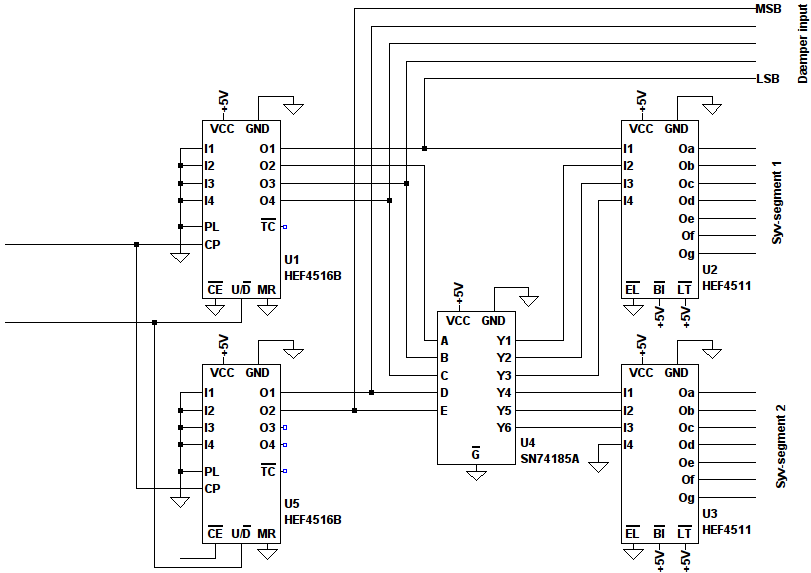
\includegraphics[width=\textwidth]{teknisk/volumenkontrol/taeller.png}
\caption{Diagram over tælleren og displaydriveren}
\label{fig:taeller}
\end{figure}

Det er tællerens opgave at holde styr på hvad volumenniveauet er. Diagrammet er vist på figur \ref{fig:taeller}. Der tælles op eller ned når der trykkes på én af de to volumenknapper. Hvor hurtigt der skal tælles bestemmes af det AND'ede signal fra VCO'en og XOR-gaten. VCO'en fungerer som en clock på AND-gaten, mens XOR-signalet sørger for, at det kun er den ene knap der holdes nede. Hvis begge knapper holdes nede, vil XOR-signalet være lavt, og der vil intet signal blive sendt til tælleren. Om der skal tælles op eller ned, styres af et signal fra vol- knappen. Hvis denne er nede, som den eneste knap, vil tælleren tælle ned af. Hvis denne ikke er nede, men XOR-signalet stadig er højt, betyder det at den anden knap er nede og tælleren vil derfor tælle op. Tælleren giver et binært output, som danner grundlag for hvad der vises i displayet og hvordan reguleringen af volumen indstilles. Tælleren der benyttes er en 4-bit tæller af typen HEF4516B. Da fire bit ikke er nok skal der bruges to. Yderligere skal der også bruges noget kontrol logik, det er for at sikre tælleren ikke tæller for højt eller lavt og for at styre den anden tæller.

\subsection*{Display}
\label{volumenkontrol-design-display}
Indstillingen af volumenkontrollen vises på to 7-segmenter. Dette er valgt, fordi disse er enkle at styre med simple kredsløb og det derfor ikke er nødvendigt med en microcontroller for at styre dem, som tilfældet havde været, hvis et LCD-display i stedet var blevet benyttet.

\subsection*{Displaydriver}
\label{volumenkontrol-design-display_driver}
Displaydriveren konverterer signalet fra tælleren til et signal der kan vises på de to 7-segment displays. Diagrammet er vist på figur \ref{fig:taeller}. Der konverteres fra tællerens binære output til BCD, Binary-coded decimal, for så at konvertere det til et signal 7-segment displayne kan vise. Der benyttes en SN74185A til konverteringen fra binær til BCD. Fordelen ved at konvertere til BCD først er at denne konvertering også deler det binære tal op i to, enere og tiere. Disse to binære tal sendes igennem en 7-segmentsdriver, HEF4511, for at få et output der fungerer med 7-segmenterne.

\subsection*{Dæmper}
\label{volumenkontrol-design-daemper}
Dæmperen er en en analog attenuator, der er sammen sat af to sæt modstands attenuatore hver efterfulgt af en buffer. Dæmpningen indstilles ved at ændre hvor signalet tages ud af de to modstands attenuatore, dette styres med en analog multiplekser. Den første attenuatorer består af syv modstande hvor der er en dæmpning på 8 dB mellem hver, den anden attenuatorer består af otte modstande hvor der er en dæmpning på 1 dB mellem hver. Det er således muligt at kombinere de to attenuatorer til at dæmpe signalet mellem 0 og 55 dB, med spring af 1 dB. Diagrammet er afbilledet på figur \ref{fig:volumenkontrol_daemper}. Modstandene er beregnet i appendiks C??.

\begin{figure}[h]
\centering
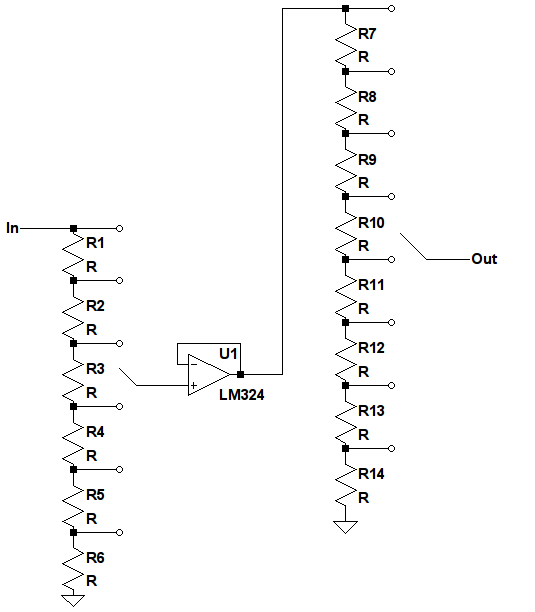
\includegraphics[width=\textwidth]{teknisk/volumenkontrol/daemper.png}
\caption{Diagram over dæmperen}
\label{fig:volumenkontrol_daemper}
\end{figure}

\section{Simulering}
\label{volumenkontrol-simulering}

Som det ses på figur \ref{fig:vco-signal} svinger udgangen på integratoren mellem schmidt-triggerens to niveauer. Det kan også ses udfra grafen hvornår VCO'ens udgang er høj, dette er når integratorens udgang, den blå kurve, er højere end $U_{6_{\mathrm{in+}}}$, den røde kurve.

\begin{figure}[h]
\centering
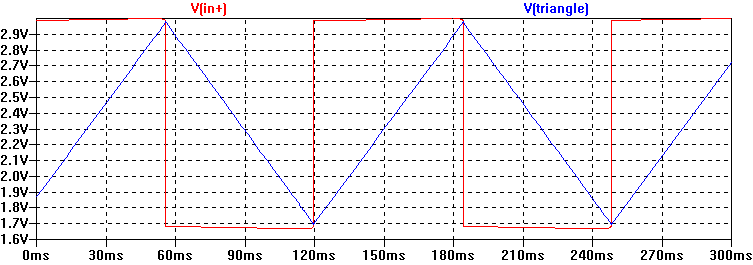
\includegraphics[width=\textwidth]{teknisk/volumenkontrol/vco-signal.png}
\caption{Integratorens udgang og $U_{6_{\mathrm{in+}}}$}
\label{fig:vco-signal}
\end{figure}

\section{Accepttest}
\label{volumenkontrol-accepttest}

